\documentclass[sigconf, nonacm]{acmart}

\begin{document}
\title{Efficient Selection of Time Series Shapelets}

%\author{Adam Charane}
%\affiliation{%
%\institution{Free University of Bozen-Bolzano}
%\city{Bolzano}
%\state{Italy}
%}
%\email{acharane@unibz.it}

%\author{Matteo Ceccarello}
%\affiliation{%
%\institution{University of Padova}
%\city{Padova}
%\state{Italy}
%}
%\email{matteo.ceccarello@dei.unipd.it}

%\author{Johann Gamper}
%\affiliation{%
%\institution{Free University of Bozen-Bolzano}
%\city{Bolzano}
%\state{Italy}
%}
%\email{johann.gamper@unibz.it}


\newcommand{\mc}[1]{\textcolor{teal}{ --- MC: #1 --- }}
\newcommand{\ac}[1]{\textcolor{orange}{ --- AC: #1 --- }}
\newcommand{\jg}[1]{\textcolor{red}{ --- JG: #1 --- }}


%%
%% The abstract is a short summary of the work to be presented in the
%% article.
\begin{abstract}
	Praesent imperdiet, lacus nec varius placerat, est ex eleifend justo, a vulputate leo massa consectetur nunc. Donec posuere in mi ut tempus. Pellentesque sem odio, faucibus non mi in, laoreet maximus arcu. In hac habitasse platea dictumst. Nunc euismod neque eu urna accumsan, vitae vehicula metus tincidunt. Maecenas congue tortor nec varius pellentesque. Pellentesque bibendum libero ac dignissim euismod. Aliquam justo ante, pretium vel mollis sed, consectetur accumsan nibh. Nulla sit amet sollicitudin est. Etiam ullamcorper diam a sapien lacinia faucibus.
\end{abstract}

\maketitle


\section{Introduction}
Time series classification is similar to traditional classification where the
difference is that the order of the values of the time series is crucial, since
it holds discriminatory features of the time series. The literature is rich of
algorithms for classifying time series, and one way to group them,
suggested by Bagnall et al.~\cite{bake_off}, is based on the techniques that
each algorithm uses to exploit the discriminatory features:
\begin{itemize}
	\item Distance based: Classification is based on using distance measures to
	      the raw time series.
	\item Feature based: Global features are extracted and the data is transformed
	      from the time domain to the feature domain spanned by the extracted
	      features, and the classification is done using a standard classifier.
	\item Interval based: Techniques in this family extract one or more intervals,
	      then statistical summaries of these intervals are used as features.
	\item Shapelet based: This technique exploits discriminatory patterns that
	      appear in time series of the same class.
	\item Dictionary based: These algorithms use as features the count of
	      repeating patterns.
	\item Convolution based: Features used are extracted from time series using
	      convolutions and pooling operations.
	\item Deep learning: Classification is done by feeding the data to neural
	      networks
	\item Hybrid: Algorithms in this category combine two or more approaches from
	      the previous techniques.
\end{itemize}
Our focus in this paper is on extracting discriminating patterns, i.e. shapelets
that represent time series from each class. The extracted patterns then can be
used by algorithms from the shapelet based technique in order to execute the
classification task.

Time series classification using shapelets is usually done over three phases:
\begin{enumerate}
	\item Extraction of candidates~\cite{keogh_shapelet, random_shapelets, fss}:
	      Select subsequences that can be used as discriminating patterns.
	\item Evaluation of the candidates~\cite{alternative_measures,
		      shapelet_transform, silhoutte_shapelets}: Compute some statistics
	      about the extracted patterns in order to rank and select the best
	      ones (the most discriminating).
	\item Data Transformation~\cite{shapelet_transform}: After the best
	      candidates are chosen, the time series have to be transformed to a
	      format that can be used by standard classifiers.
\end{enumerate}
The extraction step can be done in different ways such as considering all the
subsequences. However, this results in high number of candidates. Namely, given
a dataset of $m$ time series each having a length $n$, then the number of
candidates considered is in the order of $\mathcal{O}(n^2m)$. Another popular
alternative is to randomly select subsequences from different time series and
from different positions. Another new approach is based on selecting
subsequences based on some statistics that can be computed efficiently such as
rolling mean, variance, change in the slope or other simple statistics.

Extracting candidates by itself can be done efficiently, but the challenge is
the second step, as the evaluation is based on the similarity between the
candidates, or between the candidates and the time series. For instance, if the
candidates are extracted using brute force(considering all the subsequences)
then computing evaluation statistics would require computing distances between
all pairs which is in the order of $O(n^4m^2)$. Clearly, this is very
inefficient and becomes impossible for even relatively small datasets.

Instead of evaluating by giving a score to each candidate independently, our
approach use efficient similarity search indexing approaches and exploits the
similarity structure in order to select the best candidates. The idea is that
good shapelets representing a class $C$ should have a lot of nearest neighbors
that are from the same class, and at the same time, should have few or no
neighbors from other classes.


\section{Background \& Related work}
In a classification setup, the idea of a shapelet, introduced by Ye and
Keogh~\cite{keogh_shapelet}, is that time series from the same class must have
some shared pattern that is similar to all of them and less similar to time
series from other classes. A pattern is simply a subsequence of the time series,
and the (dis-)similarity is a distance measure, usually the normalized Euclidean
distance. Besides the high accuracy of shapelets, they are also interpretable,
since the subsequences chosen as shapelets can be interpreted as the event that
happened at that period of time.
Although the idea being simple, it introduced many challenges. The two
challenges we are concerned about are:
\begin{enumerate}
	\item How to choose patterns?
	\item How to evaluate them?
\end{enumerate}
In the original work~\cite{keogh_shapelet}, the authors considered all the
subsequences as patterns, and for the evaluation part, they ranked the patterns
by assigning to each a score. The score was the information gain, which is based
on the Shanon entropy, before and after considering the subsequence. At the end,
only the subsequences with the highest score were selected as shapelets.
Despite that only few patterns were selected, they all had to be evaluated,
which means, the similarity between all of them had to be computed in order to
assign a score. Computing the similarity was the bottleneck of the computation,
in order to speed it up, the authors had to apply early computation pruning.
The pruning resulted in a speed up, but still the approach is very slow,
and not practical for medium and large size datasets. To improve the running
time, random selection of shapelets~\cite{random_shapelets} have been
introduced. The authors empirically shown that by selecting a large number of
shapelets, i.e., by randomly selecting subsequences with different lengths from
random time series at random positions, the computation becomes much faster
since only few patterns are considered, while the accuracy remains competitive.

In order to speed up the selection process, Ji et al.~\cite{fss} introduced
Fast Shapelet Transform (FSS), that works on two different steps. First, they
sample  time series with the help of subclass splitting. This reduces the
number of time series to be considered significantly, without affecting the
accuracy, since the goal is to look for similar patterns and not all patterns.
Second, the Local Farthest Deviation Points (LFDP) are selected and used as the
endpoints of the subsequences. An LFDP is the point that has the largest
distance from the subsequence fitting line. The intuition is that the constant
subsequences should be ignored and only subsequences where there are changes
should be interesting.

Regardless of the technique used in order to select the candidates, the
evaluation in the above approaches was done using the information gain.
Lines et al.~\cite{alternative_measures} were the first to consider using
different evaluation methods instead of the information gain. They considered
as evaluation measures statistical tests to verify if points from the same
distribution or not, such as Kruskal Wallis and Mood's medians. On another
the same authors use the ANOVA F-statistic~\cite{shapelet_transform} as an
evaluation measure, which was not significantly better than the information
gain, but on average, shapelets selected using the F-statistic resulted in high
classification accuracy.
A recent work~\cite{silhoutte_shapelets} proposed the usage of Silhouettes
\cite{silhouettes} as an evaluation measure, the results were competitive with
the F-statistic and information gain, but the silhouette had much better results
when the number of shapelets used to classify was small.

While all the previous work found shapelets by extracting subsequences from the
time series, Grabocka et al.~\cite{learning_shapelets} take an alternative
approach, where instead of selecting shapelets, they \emph{learn} them by
solving an optimization problem.


\section{Preliminaries}
This section defines the key concepts used in the paper.
\begin{definition}[Time Series]
	A time series $T$ is sequence of $n$ consecutive real numbers:
	$T = [T_1, T_2, \dots, T_n]$.
\end{definition}

\begin{definition}[Subsequence]
	A subsequence of length $l$ from a time series $T$ starting from position $i$
	is an ordered set of consecutive values from $T$ denoted as:
	$S_{i, l} = [T_i, T_{i+1},, \dots, T_{i+l-1}]$.
\end{definition}

\begin{definition}[Sliding window]
	A sliding window of length $l$ over a time series $T$ is the set of
	all subsequences of length $l$ extracted from $T$:
	$W_T^l = [S_{1, l}, S_{2, l}, \dots S_{n-l+1, l}]$.
\end{definition}

A dataset consists of $m$ time series, each having a class label $c \in [1, 2,
		\dots, K]$. The sliding windows $W_T^l$ all have the same class label $c$ of the
time series $T$ they were extracted from. To compute the evaluation score of
each window using the Silhouette, we need first to introduce a (dis-)similarity
measure. In this work, we consider the normalized Euclidean distance:

\begin{definition}[Normalized Euclidean distance]
	The normalized Euclidean distance between two subsequences $S$ and $Q$ of
	length $l$:
	$$d(S, Q) = \sqrt{\sum_{i=1}^l (\frac{S_i - \mu_S}{\sigma_S} - \frac{Q_i -
				\mu_Q}{\sigma_Q})^2}$$
	where $\mu_S$ and $\sigma_S$ represent the mean and standard deviation of
	$S$ respectively.
\end{definition}

Finally, we define the silhouette score for a subsequence:

\begin{definition}[Silhouette score of a subsequence]
	Given a set $\mathcal{D}$ of subsequences (sliding windows) and their
	corresponding labels, the silhouette score for a subsequence $S_i$ having label
	$c$ is:
	$$
		s(S_i) = \frac{b - a}{\max{(a, b)}}
	$$
	where:
	\begin{itemize}
		\item $a = \frac{\sum_{k \in I_c}d(S_i, S_k)}{|I_c|}$,
		\item $b = \frac{\sum_{j \in I \setminus I_c}d(S_i, S_j)}{|I \setminus I_c|}$,
		\item $I$ is the set of indices of all subsequences in $\mathcal{D}$, and
		\item $I_c$ is the set of indices of subsequences having label $c$.
	\end{itemize}
\end{definition}

Notice that our definition of the silhouette, the term $b$ considers all
subsequences from other classes instead of only considering only the class that
is closest to the subsequence $S_i$. Next, a fixed number of subsequences from
each class are selected as shapelets, based on the highest score achieved.


\section{Approach}
The bottleneck of the computation is in the evaluation part, where, in order to
compute the Silhouette score (same for the F-statistic and the other measures),
all pairs of distances have to be computed. To avoid that, we will use the fact
that shapelets with a high silhouette score are of good quality for time
series classification. Since in a clustering setup, silhouette index of a
cluster is high when the cluster is compact and far from other clusters, and
the silhouette score of a cluster is simply the average of the silhouette
scores of the subsequences in that cluster, then the subsequences with high
silhouette are contained in the cluster.

\subsection{Clustering-based shapelets}
\begin{figure*}
	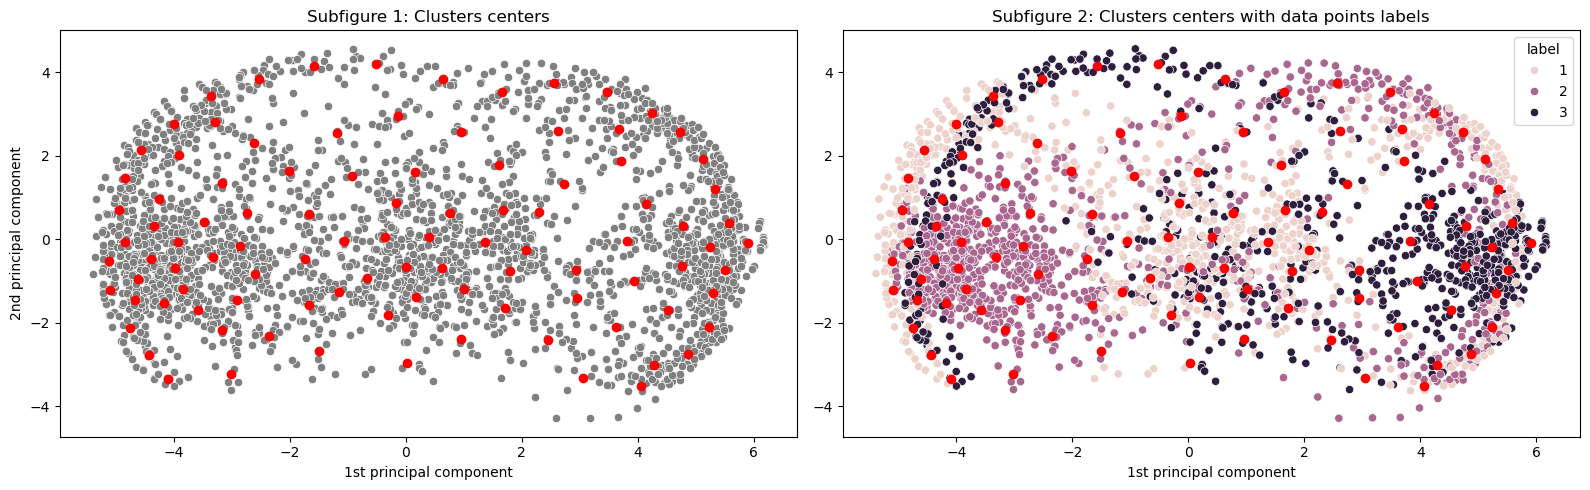
\includegraphics[width=\textwidth]{imgs/clustering.png}
	\caption{Sliding windows of length 40 from \emph{CBF} dataset, with centers
		(red dots) of 100 clusters using K-Means algorithm.\label{fig:clustering}}
\end{figure*}
We start by extracting the set of sliding windows $W$ from all the time series
$W = \bigcup_T W_T^l$, then we cluster all the windows in $W$.
For each cluster $C_i$, we count the fraction of windows from each class
(popularity), and only keep clusters where the popularity of one class is beyond
a threshold. Figure~\ref{fig:clustering} shows an example from the \emph{CBF}
dataset plotted on the plan by keeping only the first two PCA components. The
gray dots in the left sub-figure are the windows of length 40, and the red dots
are the centers of the clusters obtained y running K-Means algorithm with 100
clusters. The right sub-figure shows the labels of the subsequences.
Figure~\ref{fig:clustering_threshold} shows the same windows, but this time
after removing all the clusters where the popularity of the dominant class is
below some certain threshold.
The idea is that we want to get rid of all subsequences from different classes
that are similar to each other, since a shapelet should be a pattern repeated
between time series from the same class. Notice that the threshold might have a
high impact on the results, since when we apply a $90\%$ threshold, we have lost
some important clusters for class 2 (top right in Figure
\ref{fig:clustering_threshold}, as well as some clusters for class 1 (in the
middle of the plot).
\begin{figure*}
	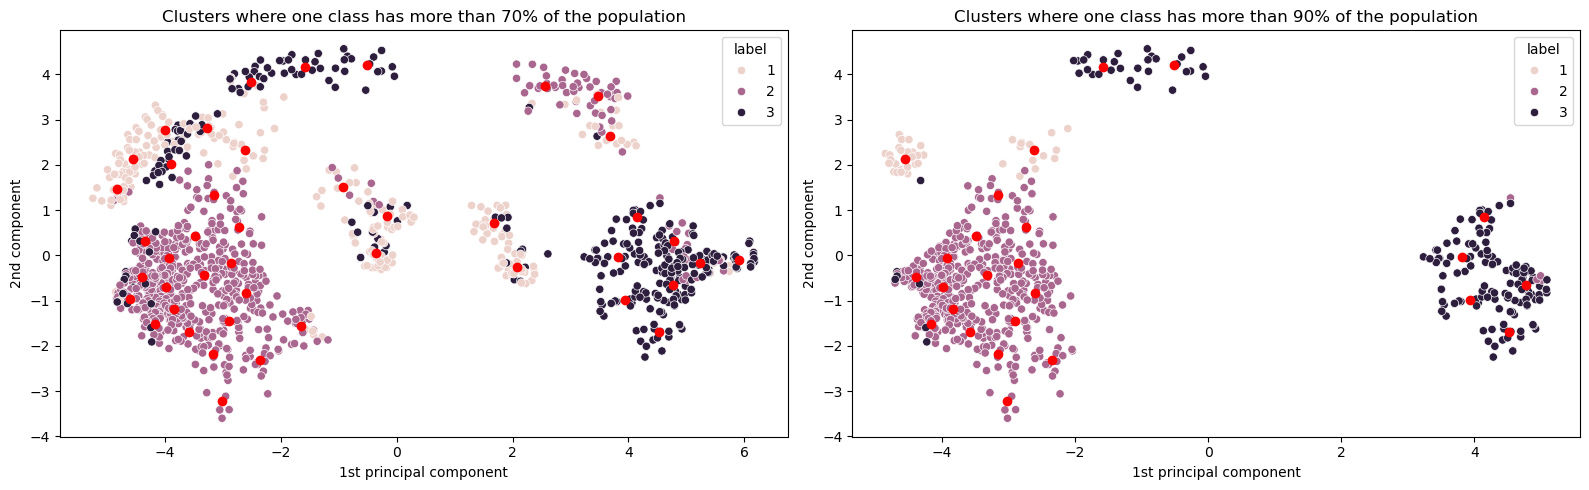
\includegraphics[width=\textwidth]{imgs/clustering_thresholds.png}
	\caption{Windows left after removing all the clusters where the popularity of
		the dominant class is below a threshold\label{fig:clustering_threshold}.}
\end{figure*}

\ac{
	There are many questions/decisions that have to be made:
	\begin{itemize}
		\item How many clusters we should use?
		\item Which clusters to keep (so far I am using the popularity)?
		\item Another approach would be to select top clusters from each class. This
		      is especially relevant when a class is never dominating in terms of
		      population, that is, if we put a threshold, there are no clusters
		      where a class $c$ has more than the threshold of the population, then we
		      will end up with no shapelets representing a specific class.
		\item Should we use all the clusters kept?
	\end{itemize}
	Some information that we have and that have not been used yet:
	\begin{itemize}
		\item In each cluster, besides the popularity of each class, we know also
		      how many time series are covered. For example, in the \emph{CBF}
		      dataset, we have 30 training examples, 10 for each class. If we have
		      two clusters with popularity, let's say 90\% for class 1, the windows
		      from cluster 1 are all extracted from 2 time series, and in the second
		      clusters, the windows are from all 10 time series, clearly we have to
		      favor the second cluster, since it has a pattern that is repeated
		      between all the of the time series from the same class. How can we
		      use this information?
		\item How to use the distance between the centers of the clusters?
	\end{itemize}
}

\subsection{Similarity search indexing-based shapelets}
In the previous subsection, we have used clustering to get rid of the evaluation
part and reduce the computational overhead. We used clustering because it is the
first intuitive idea in order to optimize for the silhouette score.
Since what we care about is the structure of similarity search, i.e., we want to
know, for each subsequence, which other subsequences are the most similar. An
alternative approach to answer these questions, one can use efficient indexing
data structures from the nearest-neighbor problem literature, which is more
efficient compared to clustering in terms of time complexity and running time.

\section{Experimental Evaluation}
In this section we compare the running time and the accuracy of our two
approaches with the baselines, namely:
(1) Ultra fast shapelet transform, which randomly select shapelets, evaluate
selects the ones with the highest rank. (2) Learning shapelets. (3) Fast them,
and Shapelet Selection (FSS).


\section{Conclusion}


\bibliographystyle{ACM-Reference-Format}
\bibliography{bibliography}

\end{document}
\endinput
